\chapter{多类生物标记物定位问题实验评估}\label{sec:multi_classes}
\section{前言}
本章
\section{数据集介绍}
\subsection{多类模拟皮肤病病变数据集}
多类模拟皮肤病病变数据集同样是包含带有人工生物标记物的皮肤图像,图像尺寸大小均为$128\times 128$,图像均以PNG格式存储,每张图像不仅有图像级标注,还有像素级标注,可用于定量分析有关的实验评估。在\ref{subsec:bin_simulated_skin_ds}小节中用到的二类模拟皮肤病病变数据集基础上额外增加了两类,故多类模拟皮肤病病变数据集中一共有$4$类,其中$3$类异常,$1$类正常。正常类图像是从ISIC2018~\cite{codella2019skin, tschandl2018ham10000}分类任务中的图像\footnote{https://challenge2018.isic-archive.com/task3/}通过滑动窗口方式收集$922$张正常皮肤图像(实际上是图像块)。第一类异常与二类模拟皮肤病病变数据集中的异常类一样,生成过程也相同(相关介绍参见\ref{subsec:bin_simulated_skin_ds}小节)。第二类异常图像中的生物标记物是黑色素瘤病变区域,为了生成这个数据集,我们首先从ISIC2018的分类任务(注意没有重复使用图像)提取了图像大小为$128\times 128$的正常图像(同样通过滑动窗口方式)。同时,我们根据ISIC2018的分割任务\footnote{https://challenge2018.isic-archive.com/task1/}中的黑素瘤区域的像素级标签,将其中的黑素瘤像素提取出来并嵌入到正常图像中。在此过程中,为了模拟真实皮肤图像中生物标志物的数量、大小和所在位置的随机变化,我们通过随机参数控制,在每个模拟皮肤图像的一定范围内随机生成这些参数的值。具体来说,黑色素瘤病变区域尺寸大小为$8\times 8$、$10\times 10$、$15\times 15$、$20\times 20$或者$25\times 25$。另外,为了产生不规则形状的生物标记物,对于每个缩略图的每个像素,以$1/3$概率不填充黑色素瘤像素。另外,我们还设置每张正常图像中嵌入的缩略图的数量不同($1$到$3$张)。第三类异常图像与第一类异常图像生成方法相同,只是第三类异常图像中的生物标记物不再是Image-Net图像的缩略图,而是圆环。最终,正常类、第一、二、三类异常中分别有$922$、$1,310$、$1,051$、$1,062$张样本。
\begin{figure}[h]
	\centering
	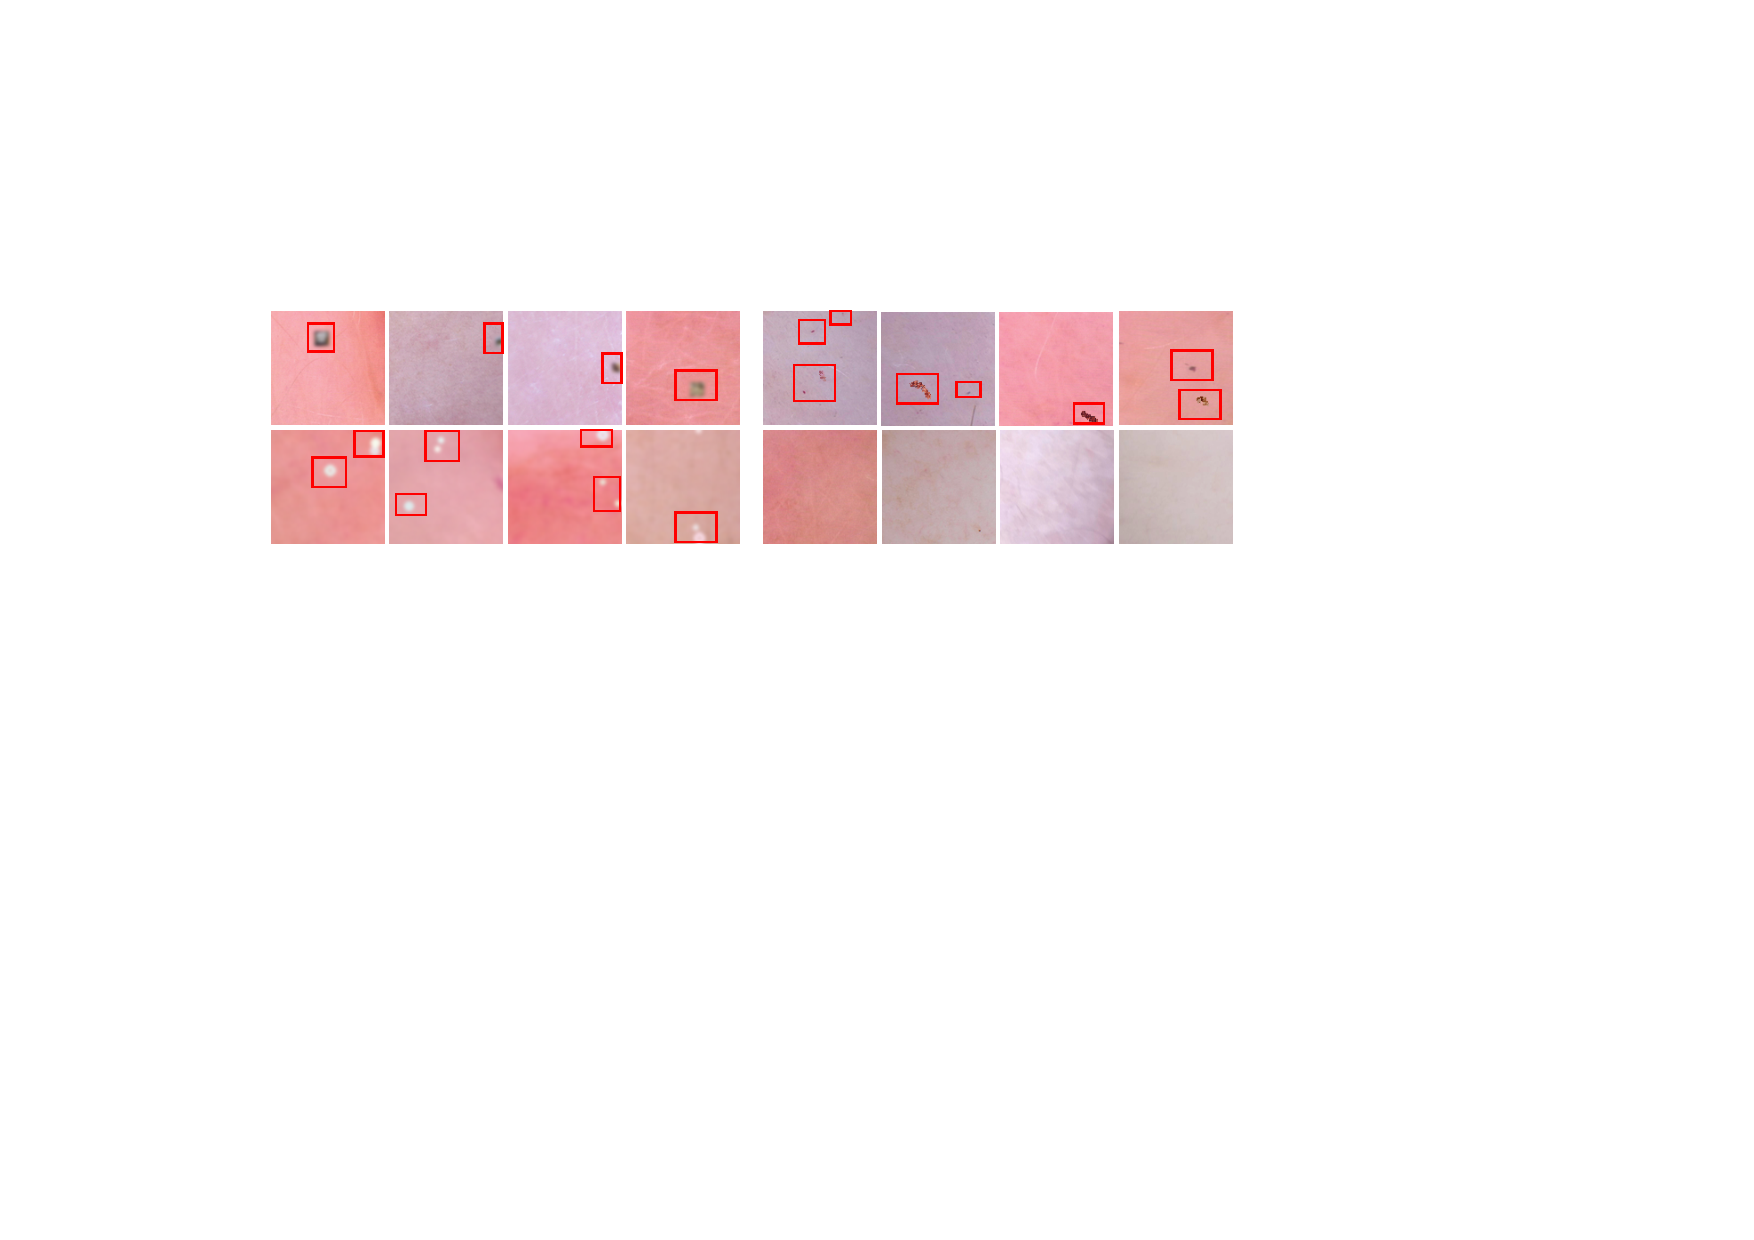
\includegraphics[width=1.0\textwidth]{figure/multi_classes_simulated_skin.pdf}
	\caption{多类模拟皮肤病病变数据集图像示例:按照从上到下,从左到右的顺序,第$1$行第$1$列到第$1$行第$4$列为皮肤图像加上经过局部模糊的Image-Net缩略图的异常图像;第$1$行第$5$列到第$1$行第$8$列为皮肤图像加上黑色素瘤区域的异常图像;第$2$行第$1$列到第$2$行第$4$列为皮肤图像加上经过局部模糊的圆环区域的异常图像;第$2$行第$5$列到第$2$行第$8$列为正常图像。异常图像中的生物标记物均已用红色矩形框标出。}
	\label{fig:mul_classes_simulated_ds}
\end{figure}

\section{实验设置}
\section{在多类生物标记物定位问题实验评估}
\begin{figure}[h]
	\centering
	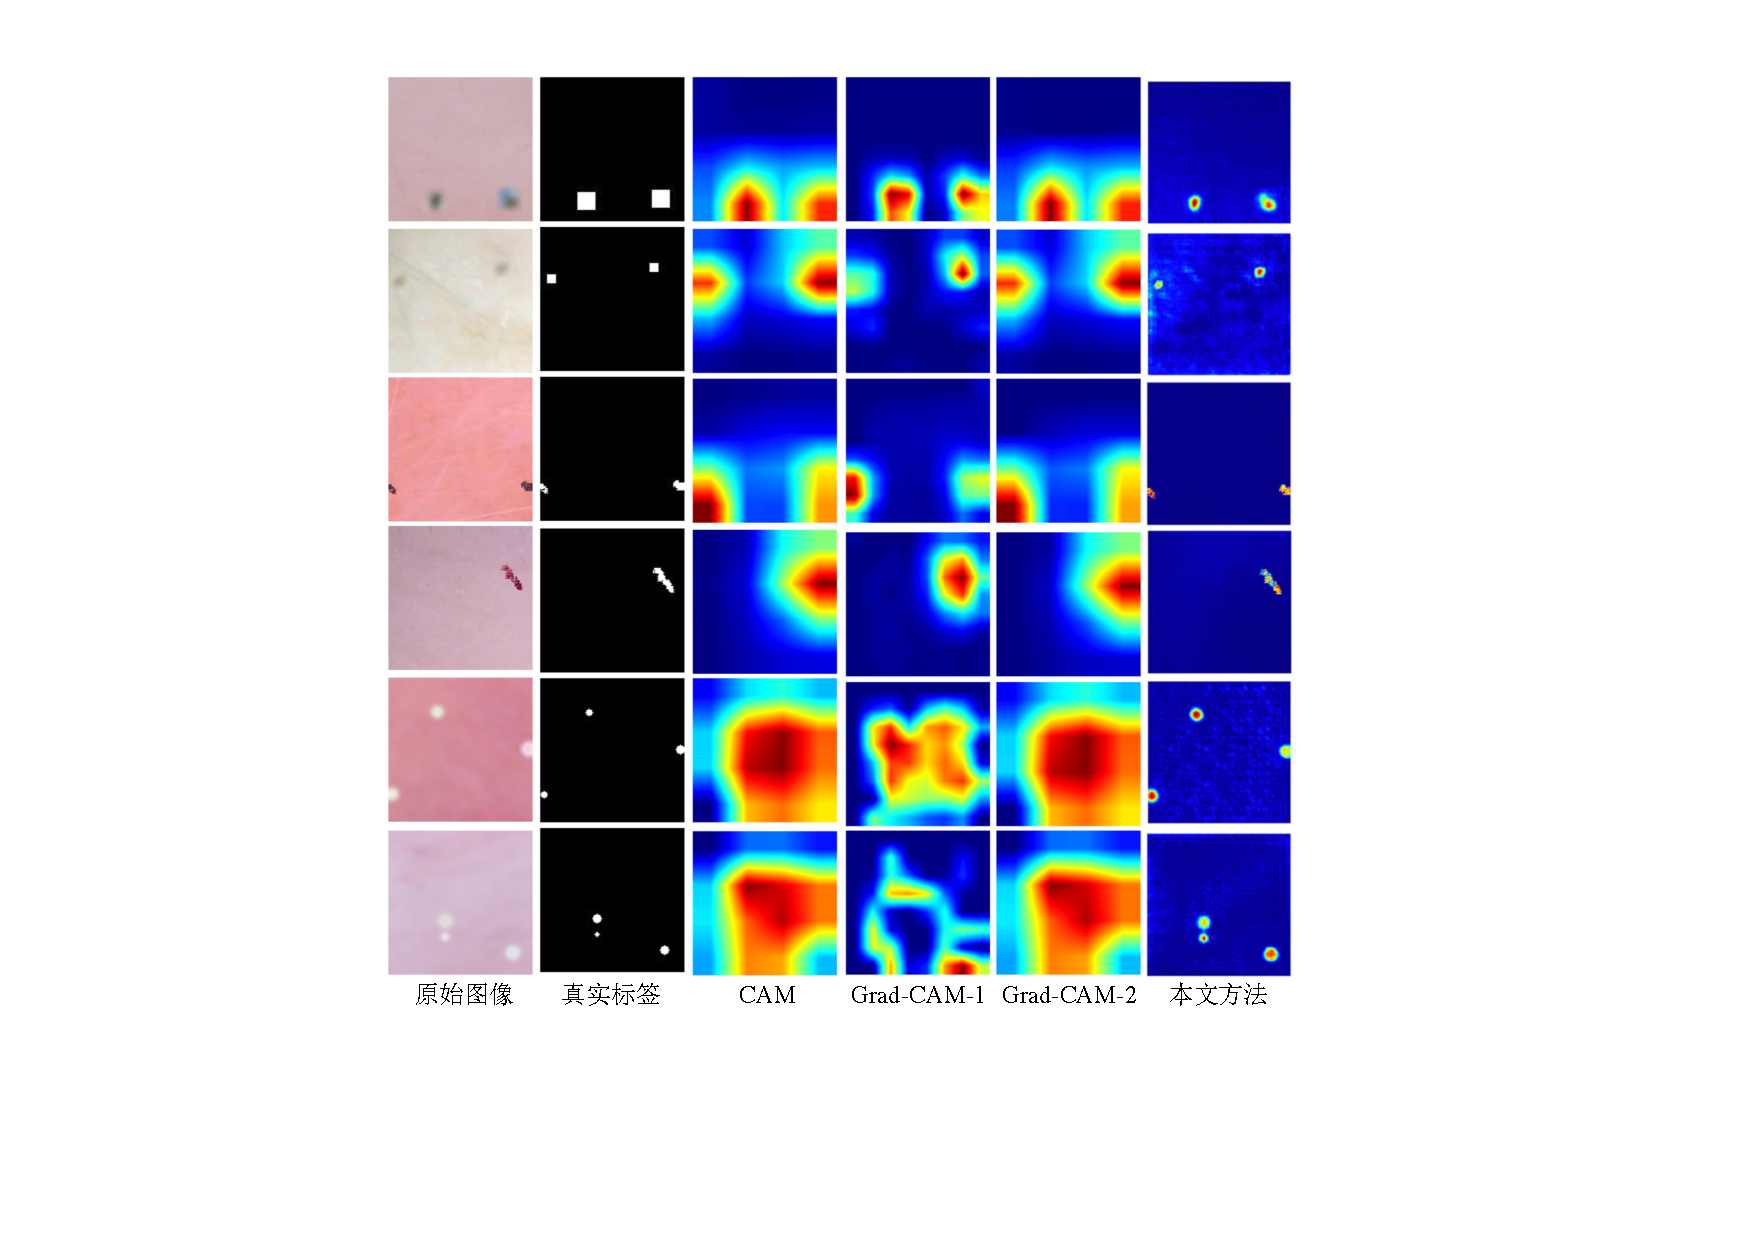
\includegraphics[width=1.0\textwidth]{figure/multi_simulated_skin_res.pdf}
	\caption{}
	\label{fig:multi_simulated_skin_res}
\end{figure}
\section{对于经过编码器-解码器的多类模拟皮肤病病变图像的定量分析}
\section{不同超参数下的实验结果分析}
\section{对判别器模型结构的探究}
\section{本章小结}
